\chapter{Metaphor and Coercion} \label{chap:figurative}
In this chapter, I will extend the empirical work on exploring the application of my context sensitive distributional semantic models to two semantic phenomena which involve the application of words in situations where their meanings are in some sense conceptually altered: \emph{metaphor} and \emph{semantic type coercion}.  The precise definitions of these terms, which are not without nuance, was explored in Chapter~\ref{sec:figurative} and will be reintroduced in subsequent sections.  As an overview, the distinguishing characteristic of these phenomena is that they involve cases where what might be thought of as the stable, encyclopedic understanding of some word sense -- a \emph{dictionary definition} of a word, so to speak -- is in some way appropriated or subverted in order to, among other things, transfer information via the attributional conduits connecting figurative source to literal target.

My hypothesis is that, because figurative language always involves the contextual specification of word meaning, context sensitive geometries of lexical representations should provide an appropriate framework for identifying when this type of semantic phenomenon is in effect.  \cite{Fraser1993} demonstrates empirically that metaphor interpretation is, when a metaphor is presented to a subject out of context, an ambiguous exercise, and, to the extent that interpretations of de-contextualised metaphors can be predicted, the predicting factors are themselves culturally relative.  Along similar lines, \cite{BouveretEA2009} propose that metaphor production involves the contextual alignment of overlapping semantic frames, and that this alignment likewise imports structure associated with one frame into the domain of another, evident in, for instance, the additional transposition of syntactic constraints from source to target.  From a cognitive perspective, this coordinates a contextual theory of metaphor with the work on conceptual frames from \cite{Barsalou1992,Barsalou1993} discussed at the end of the previous chapter in the context of judgements of semantic similarity.  From a modelling perspective, this suggests that a methodology for projecting semantic spaces where context specific perspectives can reveal \emph{ad hoc} perspectives on semantic relationships should be a productive approach to identifying figurative language.

The idea that metaphor and metonymy are both instances of ``a connection between two things where one term is substituted for another,'' \citep[][p. 260]{Gibbs1993} will quickly call to mind the premise of distributional semantics: if the motivation for building vector space models of word co-occurrence statistics is that related words have similar co-occurrence tendencies, then figurative language might be construed as a special case in which unrelated or at least conceptually divergent words are likewise found in similar sentential situations.  The question, then, is whether statistical characteristics of the particular co-occurrences profiles selected by words with different meanings are predictive of figurativeness.  A naive hypothesis might be that word combinations that are figurative should simply be further apart in a semantic space than word combination that are literal.  If related words have similar co-occurrence profiles, then maybe unrelated words, for instance words with different conceptual entailments, should have less similar co-occurrence profiles.  This conjecture, however, is belied first of all by the fact that, in the type of corpus containing a broad range of examples of language use necessary for building distributional semantic models, figurative language will already be built into the data (and at the end of this chapter I will argue, in line with, for instance, \cite{Gibbs1994}, that figurative language is going to built into any sample of language no matter how small or basic).  A second problem is that, specifically to overcome the problems with modelling semantic relationships merely in terms of collocations, distributional semantics compares the co-occurrence profiles of words rather than their direct relationships, and it seems likely that word combinations prone to metaphoric interpretation might very well have at least overlapping profiles.

So the objective of the experiments reported in this chapter will be to explore the ways in which and the degrees to which a more fleshed out statistical description of contextually selected distributional semantic subspaces can reveal figurative language.  As with the experiments on relatedness and similarity reported in the previous chapter, in addition to the relationship between target word-vectors in the subspaces they select, the statistical properties of the selected dimensions themselves will also be examined.  And, again as with previous results, the instrument of analysis will be the geometric features of the subspaces in question, with, again, particular attention paid to the way in which the sets of features can collectively indicate figurative language.  The two primary datasets explored represent binary decisions about metaphoricity and coercion respectively, and so my models will be applied to classification tasks here.  In the case of metaphor, I test whether a model learned based on classification data is generalisable to graduated human ratings of metaphoricity.  With the coercion data, I will examine whether the addition of information about sentential context enhances the classification of word pairs.  I will conclude the chapter with a reflection on some of the theoretical implications of the strongly positive results described here.

The study of why humans use figurative language has a considerable scholastic pedigree.

It has served as something of a bafflement to logical empiricists from 

\section{An Experiment on Metaphor}
As pointed out by \cite{ShutovaEA2013}, statistical approaches to metaphor identification and interpretation have generally been formulated in the context of the \emph{conceptual metaphor} theory of \cite{LakoffEA2003}.  This model is founded on the principle that ``we systematically use inference patterns from one conceptual domain to reason about another conceptual domain,'' (ibid, p. 246).  Metaphors are then the mechanism for performing the mapping between these domains, and as such cut right to the core of cognitive processes.  Statistical models of metaphor have accordingly treated metaphors as transformations of lexical representations, and vector space models of distributional semantics have naturally leant themselves to this type of approach.  The construction of representations with the potential to interact with one another in semantically productive ways has in turn lent itself to the development of models that consider the compositional nature of metaphor, effectively treating the metaphor itself as a transformation of the underlying representations.  So \cite{Utsumi2011} constructs candidate metaphor-vectors by calculating the centroid of a number of vectors derived from an analysis of a noun-vector and a predicate-vector learned through latent semantic analysis, and then uses the spatial relationships between these composed vectors to analyse the metaphoricity of certain phrases.  \cite{HovyEA2013} similarly consider composition in their approach to metaphor classification, in this case by combining word-vector type representations with a model trained to identify metaphor based on dependency trees of sentences labelled for metaphoricity.

In the tradition of work on compositional distributional semantics explored by the likes of \cite{MitchellEA2010}, \cite{BaroniEA2010}, and \cite{CoeckeEA2011}, among others, semantic types such as adjectives and verbs are modelled as tensors which perform transformations on nouns, which are modelled as vectors.  In the normal run of things, compositional models therefore represent, for instance, noun phrases modified by adjectives as the product $A\overrightarrow{n}$, where $A$ is a matrix representing an adjective learned from observations of attested instances of the adjective with other noun word-vectors.  So the phrase \emph{black dog} becomes a word-vector in the same space as the representation of just \emph{dog}, and can be compared quantitatively and geometrically with other phrases such as \emph{white dog} or \emph{big cat} and so forth.  In the case of metaphor, these transformations are expected to map the word-vector representing metaphoric phrases into a region corresponding to the semantic domain of the original noun-vector modified by a metaphoric interpretation of the word associated with the tensor of a modifier or a predicate.  So, for instance, in a model that effectively captures metaphoricity, the composition of the vector space representations corresponding to \emph{brilliant light} would map to a region of space where comparisons between phrases like \emph{dark illumination} and \emph{red glow} are productive, while \emph{brilliant child} might be expected to map into the proximity of \emph{stupid boy} and \emph{boring girl}.\footnote{It should be noted that such a methodology at this point begins to assume dim shades of \citepos{Gardenfors2000} conceptual spaces, with different compositions inherently defining different regions of the space.}

The data that I will use in this section to test my methodology was originally presented by \cite{GutierrezEA2016}, along with an accompanying experiment on a novel model.  It consists of 8,592 adjective-noun pairs, spanning 23 adjectives chosen for their membership in six different broad semantic categories that are prone to both literal and metaphoric use: so, for instance, \emph{bitter}, \emph{sour}, and \emph{sweet} are considered constituents of the category \textsc{taste}.  There are 3,473 different noun types used, with only 141 types, represented by 640 tokens, occurring in both literal and metaphoric phrases.  Each pair has been rated as either literal or metaphoric by a pair of human annotators, with inter-annotator agreement measuring at Cohen's $\kappa = 0.80$; 4,593 of the pairs have been judged metaphorical.  This dataset was conceived as something of an expansion of the similar but smaller corpus of adjective-noun phrases annotated with binary metaphoricity classifications presented by \cite{TsvetkovEA2014} (and those authors tested their own data with an assortment of models, achieving highest f-scores by applying a random forest classifier to the features of an existing library of distributional semantic word-vectors).

In their own experimental treatment of the data, \citeauthor{GutierrezEA2016} constructed a pair of compositional models in the mode of \cite{BaroniEA2010}, learning adjective matrixes $A$ to map from noun-vectors to noun-adjective phrase-vectors extracted from observations of co-occurrences of both nouns and phrases in a corpus.  By creating separate tensor representations for literal and metaphoric instances of a given adjective, the authors can then compare the relationships between the vectors resulting from a noun-vector composed with literal and metaphoric senses of an adjective-vector to try to determine whether a given phrase would generally be classified as a metaphor or a literal expression by comparing the respective compared vectors to the phrase-vector as observed in the corpus.  In a further attempt to generalise the method, and, notably, to apply the conceptual metaphor theory of \cite{LakoffEA1980} to their computational model, the authors learn matrices performing linear transformations from literal to metaphoric adjective-noun compositions and then compare the similarity between observed phrase-vectors and literal composed vectors versus transformed literal composed vectors to determine whether a given phrase is metaphoric or not.

The data described by \citeauthor{GutierrezEA2016} will serve as the basis for testing my own context sensitive distributional semantic methodology's ability to classify phrases as literal or metaphoric, and the results of this experiment will be described in the following section.  My hypothesis is that metaphor, and indeed all figurative language, is fundamentally entangled with the context mutually indicated by the representations of the words participating in the composition being analysed.  In fact, I think that part of what is captured by the model described by \citeauthor{GutierrezEA2016}, and indeed a number of other researchers investigating statistical methods for metaphor classification, is precisely that there is a context inherent in the linear algebraic dynamics of composable lexical representations, and this is something which many researchers explicitly recognise.  But I also think that the explicit projection of context specific semantic subspaces, the mainstay of my methodology, should provide an ideal testing ground to discover the way in which statistical geometry can directly broadcast the presence or absence and even potentially the degree of metaphor inherent in a given phrase.  The following sections will test this hypothesis using a similar methodology to that applied to semantic relatedness and similarity in the previous chapter.

%The section after that will explore the geometry of a particularly successful model learned using my methodology.  Finally, in Section~\ref{sec:genafor}, I will address the question of whether a classification model learned from the impressively large dataset contributed by \citeauthor{GutierrezEA2016} can be generalised to handle graduated human ratings of metaphoricity on a different type of metaphoric construction.

\subsection{Methodology and Results}
My own methodology is clearly less committed to maintaining distinct representations for different semantic types than the compositional models described above, instead modelling all words as untagged word-vectors based on their co-occurrences as observed across a large scale corpus.  This feature of my research is in part theoretically motivated: in line with \cite{Langacker1991}, and \emph{contra} the grammatic nativism or exceptionalism that has been a mainstay in theoretical linguistics \citep{Chomsky}, I would like to investigate the possiblity that ``grammar is fully and appropriately describable using only symbolic units, each having both semantic and phonological import,'' (ibid, p. 290).  In other words, the syntactic component of a natural language might be described in terms of the entanglements of the meaning-making structures -- the lexical semantic representations -- that arise in the course of language use, or maybe even as emergent properties of these entanglements.

With this in mind, I will approach the problem of metaphor classification with a similarly statistical and geometric methodology as was applied to relatedness and similarity in the previous chapter, outside of any prima fascie model of syntax or compositionality.  For every pair of words in the data produced by \cite{GutierrezEA2016}, I generate subspaces of 20, 50, 200, and 400 dimensions using the \textsc{joint}, \textsc{indy}, and \textsc{zipped} techniques, projected from 2x2 and 5x5 word co-occurrence window base spaces.  This data specifies a distince role for each word, one being a metaphoric source (the adjective) and the other being a target (the noun): so, for instance, a \emph{bitter loss} is a loss, but presumably not one with an actual loss, and so the noun \emph{loss} co-opts something of the quality of bitterness into its own conceptual domain.  As such, it might be useful to generate subspaces based simply on an anlysis of the word-vectors corresponding to the adjective and the noun respectively.  I do this by simply selecting the top $d$ dimensions, in line with the dimensionality parameter for each model, for the term in question, and these spaces are labelled \textsc{adjective} and \textsc{noun} in the results that follow.

In each subspace, I extrapolate the same 34 geometric features described in Table~\ref{tab:features} and applied in the previous chapter in the semantic relatedness and similarity experiments.  Again because of the semantic asymmetry of the relationship between the input terms, an additional seven features are also available in these spaces: the adjective-vector norm divided by the noun-vector norm ($A/B$), likewise the lengths of the vectors between the adjective and the generic points divided by the lengths for the noun-generic-point vectors ($\overline{AC}/\overline{BC}$, $\overline{AM}/\overline{BM}$, and $\overline{AX}/\overline{BX}$), and the corresponding fractions of the normalised versions of these points ($\overline{A'C'}/\overline{B'C'}$, $\overline{A'M'}/\overline{B'M'}$, and $\overline{A'X'}/\overline{B'X'}$).  These additional measures might offer a sense of wehther there are statistical tendencies that are specific to the semantic role being played by a word moving from literal to metaphorical relationships, and we might expect this to be particularly evident in the spaces selected by either the noun or the adjective on their own.

\begin{table}
\centering
\begin{tabular}{lrrrr|rrrr}
\hline
\emph{window} & \multicolumn{4}{c}{2x2} & \multicolumn{4}{c}{5x5} \\
\emph{dimensions} & 20 & 50 & 200 & \multicolumn{1}{c}{400} & 20 & 50 & 200 & 400 \\
\hline
\textsc{joint} & 0.839 & 0.860 & 0.878 & 0.881 & 0.840 & 0.862 & 0.880 & 0.886 \\
\textsc{indy} & 0.821 & 0.839 & 0.855 & 0.860 & 0.817 & 0.840 & 0.858 & 0.867 \\
\textsc{zipped} & 0.839 & 0.864 & 0.876 & 0.878 & 0.833 & 0.854 & 0.873 & 0.880 \\
\textsc{adjective} & 0.771 & 0.860 & 0.828 & 0.845 & 0.781 & 0.804 & 0.828 & 0.837 \\
\textsc{noun} & 0.819 & 0.861 & 0.843 & 0.847 & 0.806 & 0.821 & 0.838 & 0.843 \\
\textsc{SVD} & 0.685 & 0.703 & 0.703 & 0.697 & 0.677 & 0.694 & 0.687 & 0.684 \\
\textsc{SG} & 0.679 & 0.676 & 0.679 & 0.673 & 0.664 & 0.665 & 0.672 & 0.656 \\
\textsc{CBOW} & 0.669 & 0.681 & 0.677 & 0.672 & 0.669 & 0.673 & 0.677 & 0.671 \\
\hline
\end{tabular}
\caption[Context Sensitive and Static Model F-Scores for Metaphor Classification]{F-scores for metaphor identification based on a ten-fold cross-validated logistic regression taking geometric features of various subspace types as input.}
\label{tab:metaphor}
\end{table}

In order to test the capacity of the geometric features of my subspaces to identify metaphor, I perform a logistic regression taking these features as independent variables and learning to predict the classifications assigned to the word pairs in the dataset.  Balanced f-scores based on the precision and recall of my various dimensional selection techniques as well as static SVD factorisations of my base spaces and the \texttt{word2vec} models are reported in Table~\ref{tab:metaphor}.  The first hing to note is the strong performance across the board of the context sensitive methodology: the least predictive versions of my models still substantially outpoerform the strongest versions of the static models

XXX SIGNIFICANCE

The context sensitive results taking both words as input display a systematic advance as dimensionality and co-occurrence window size progress, suggesting that more information about co-occurrences, arising from larger co-occurrence windows and deeper analysis of salient co-occurrence terms corresponding to higher dimensionality, leads to more information about the likelihood of a metaphorical semantic relationship.  The \textsc{joint} technique gives the strongest results, suggesting that subspaces delineated in terms of co-occurrence dimensions mutually salient to both input terms offer the best platform for analysing metaphoricity.  This makes sense: in the case of metaphor versus literalness, it is the co-occurrences that both words have in common that position their respective word-vectors in an indicative relationship relative to one another and the subspace overall.  So for instance the co-occurrences salient to both \emph{sweet} and \emph{fruit} will have a particular conceptual profile that will not be evident in the dimensions jointly selected by \emph{sweet} and \emph{revenge}; this effect will be less evident for dimensions independently salient to each word.  \textsc{Zipped} subspaces, where there will be at least some information about both words along every dimension, accordingly score almost as well as \textsc{joint} subspaces, with the \textsc{indy} subspaces falling further behind.

Interestingly, the \textsc{adjective} and \textsc{noun} spaces classify metaphor most accurately in 50 dimensional subspaces projected from the 2x2 word window base space.  To the extent that part-of-speech can be a component of the analysis of these models, we can expect the smaller co-occurrence window to produce statistics that are more indicative of a particular grammatical class.  The degradation of classification at higher dimensionalities for the smaller co-occurrence window setting is a little surprising, and it's worth noting that the \textsc{indy} subspaces, which are basically blends of the \textsc{adjective} and \textsc{noun} subspaces, don't exhibit the same tendency.  In this case, it would seem the whole really is greater than the sum of the parts, with the dimensional selection of one word providing at least a degree of useful information about the other word not available in spaces salient to a single term.  A similar pattern emerges for the static spaces: the \textsc{SVD}, \textsc{SG}, and \textsc{CBOW} models all produce the most accurate classifications in 2x2 word window, 50 dimensional subspaces.  One way to explain this is that more ambiguous information about word use begins to leek in at higher dimensionalities, servining to obscure the more standard indications available in either the most salient dimensions or the dimensions containing the most information about variance across the corpus.

There is another possibility to consider regarding the adjectives in this dataset in particular: as there are only 23 different adjective types, each adjective is observed multiple times in both metaphoric and non-metaphoric contexts.  It is therefore possible that, in any given fold of the cross-validation of a classifier, the model might be learning how to guess whether a specific adjective is involved in a metaphor rather than something more general about the statistical geometry of metaphoricity.  In order to avoid this trap, I reorganise the data into tranches based on the adjective in each pair, I use the eight conceptual categories outlined by \cite{GutierrezEA2016} in order to structure this new partioning.\footnote{\cite{GutierrezEA2016}, identifying a similar problem, likewise develop a second model that learns metaphors as mappings between domains rather than just from noun-vectors to phrase, though their methodology requires them to use a reduced version of the data.}  I use each of these eight new sets of word pairs as a fold in a cross-validated logistic regression, such that the adjective in each phrase in each test set has not been observed in the training data.

%So it is possible that a model is detecting something about a particular adjective's propensity to be involved in a metaphor, and then learning a combination of features that effectively serve to label each adjective in a way that is mappable to a fairly reliable classification.

%Outside of my own methodology, one interesting trend to notice in these results, and in contrast to the results on relatedness and similarity discussed in the previous chapter, is that all three techniques for building static models show an ambiguous trajectory as dimensionality is increased, with in particular a slight but consistent decreases in their agreement with human classifications moving from 200 to 400 dimensional spaces.

\begin{table}
\centering
\begin{tabular}{lrrrr|rrrr}
\hline
\emph{window} & \multicolumn{4}{c}{2x2} & \multicolumn{4}{c}{5x5} \\
\emph{dimensions} & 20 & 50 & 200 & \multicolumn{1}{c}{400} & 20 & 50 & 200 & 400 \\
\hline
%\textsc{joint} & 0.817 & 0.835 & 0.842 & 0.824 & 0.825 & 0.849 & 0.855 & 0.847\\
%\textsc{indy} & 0.782 & 0.819 & 0.841 & 0.845 & 0.789 & 0.834 & 0.853 & 0.865 \\
%\textsc{zipped} & 0.804 & 0.836 & 0.844 & 0.838 & 0.819 & 0.844 & 0.864 & 0.859 \\
%\textsc{adjective} & 0.707 & 0.741 & 0.783 & 0.811 & 0.732 & 0.747 & 0.791 & 0.820 \\
%\textsc{noun} & 0.760 & 0.777 & 0.813 & 0.830 & 0.791 & 0.810 & 0.820 & 0.828 \\
\textsc{joint} & 0.815 & 0.837 & 0.854 & 0.855 & 0.816 & 0.837 & 0.858 & 0.863 \\
\textsc{indy} & 0.778 & 0.793 & 0.828 & 0.835 & 0.774 & 0.805 & 0.829 & 0.842 \\
\textsc{zipped} & 0.810 & 0.838 & 0.847 & 0.854 & 0.799 & 0.828 & 0.844 & 0.853 \\
\textsc{adjective} & 0.606 & 0.709 & 0.750 & 0.777 & 0.698 & 0.697 & 0.757 & 0.707 \\
\textsc{noun} & 0.806 & 0.808 & 0.828 & 0.833 & 0.796 & 0.812 & 0.824 & 0.829 \\
\textsc{SVD} & 0.679 & 0.691 & 0.695 & 0.690 & 0.665 & 0.674 & 0.678 & 0.676 \\
\textsc{SG} & 0.668 & 0.664 & 0.659 & 0.657 & 0.659 & 0.656 & 0.644 & 0.638 \\
\textsc{CBOW} & 0.657 & 0.665 & 0.665 & 0.661 & 0.656 & 0.660 & 0.666 & 0.660 \\
\hline
\end{tabular}
\caption[F-Scores for Metaphor Classification of Unseen Adjectives]{F-scores for metaphor identification with each of the conceptual categories identified by \cite{GutierrezEA2016} treated as a separate fold for cross-validation.}
\label{tab:categoraphor}
\end{table}

Table~\ref{tab:categoraphor} presents the results from this reshuffled version of the experiment.  The f-scores for metaphor classification returned by the context sensitive models are down slightly, but the difference is only marginally significant

XXX SIGNIFICANCE

The major change here is, as expected, in the \textsc{adjective} subspaces: clearly when only information from the adjective in each word-pair is used to train a model, prior observations of a specific word type in the context of some other composition is a benefit.  There is also a minor decrease in performance for the static models, which is interesting in that it indicates that, even when a single distance metric is used to classify metaphoricity, observations of a word in training help to subsequently test phrases involving that word.  It is worth noting that of the 8,584 noun tokens spread across 3,473 noun types, 1,588 types, represented by 6,724 tokens, occur in more than one of the tranches delineating the conceptual categorisations of the adjectives, so it is possible that there is a small extent of learning to classify phrases based on previous observations of specific nouns.

In order to take a closer look at the way that different techniques model this data, and in line with the metaphor classification work of \cite{TsvetkovEA2014}, Figure~\ref{fig:metaroc} illustrates receiver operating characteristic curves for four versions of the approaches that have been described here: the \textsc{joint} technique with 400 dimensional, 5x5 word subspaces, the same technique applied to the version of the data shuffled to avoid training and testing on the same adjectives, and the \textsc{CBOW} and \textsc{SVD} models for the optimally performing 50 dimensional, 2x2 word window subspaces.  True positive versus false positive rates are correlated at 99 increments in terms of the value of the output of a logistic regression model at which a phrase is determined to be metaphoric.  The outcomes visualised here tell a similar story to Tables~\ref{tab:metaphor} and~\ref{tab:categoraphor}, with the area under the curve statistics indicating a strong distinction between the context sensitive techniques and the static models.  Perhaps the most interesting thing to note is the overall smoothness of the curves, which suggests a steady relationship between precision and recall at various classification thresholds.

\begin{figure}
  \centering
  \footnotesize
  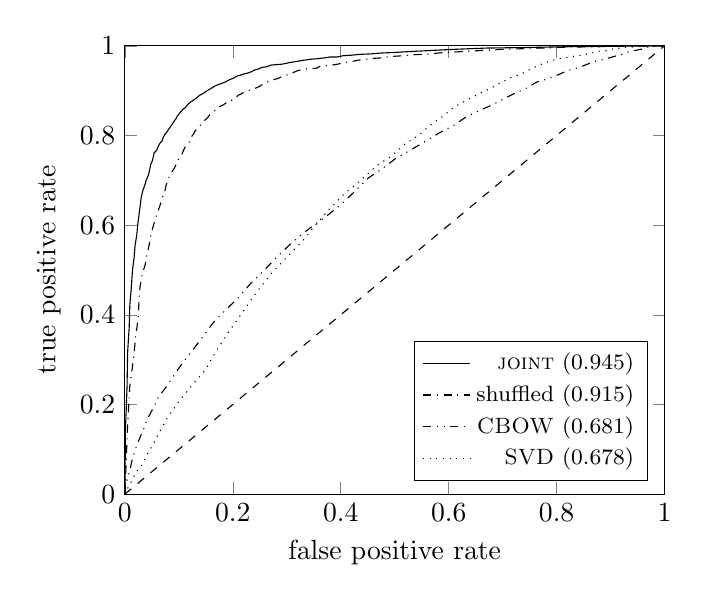
\begin{tikzpicture}
    \begin{axis}[xmin=0,xmax=1,ymin=0,ymax=1,xlabel={false positive rate},ylabel={true positive rate},legend pos=south east,legend cell align={right},legend style={font=\footnotesize}]
      \addplot [dashed,forget plot] coordinates{(0,0) (1,1)};
      \addplot [] coordinates{(0.0,0.0) (0.001,0.143) (0.004,0.240) (0.005,0.315) (0.008,0.373) (0.009,0.419) (0.012,0.463) (0.014,0.499) (0.017,0.527) (0.019,0.556) (0.022,0.578) (0.024,0.603) (0.026,0.621) (0.028,0.640) (0.030,0.660) (0.033,0.676) (0.037,0.690) (0.040,0.702) (0.044,0.713) (0.046,0.725) (0.048,0.736) (0.051,0.744) (0.053,0.754) (0.054,0.761) (0.059,0.767) (0.061,0.774) (0.065,0.783) (0.069,0.788) (0.071,0.796) (0.074,0.802) (0.078,0.808) (0.081,0.814) (0.084,0.819) (0.088,0.826) (0.092,0.833) (0.095,0.838) (0.097,0.843) (0.099,0.846) (0.102,0.851) (0.105,0.855) (0.108,0.859) (0.112,0.862) (0.116,0.868) (0.118,0.871) (0.121,0.874) (0.125,0.877) (0.128,0.880) (0.132,0.883) (0.136,0.887) (0.139,0.890) (0.144,0.893) (0.148,0.896) (0.151,0.899) (0.154,0.901) (0.157,0.903) (0.161,0.906) (0.165,0.909) (0.168,0.911) (0.174,0.914) (0.179,0.916) (0.183,0.918) (0.188,0.920) (0.190,0.922) (0.195,0.925) (0.200,0.927) (0.204,0.930) (0.209,0.933) (0.213,0.934) (0.220,0.937) (0.227,0.939) (0.234,0.942) (0.240,0.946) (0.247,0.948) (0.254,0.952) (0.262,0.953) (0.271,0.957) (0.280,0.958) (0.291,0.959) (0.299,0.961) (0.307,0.963) (0.318,0.965) (0.332,0.968) (0.345,0.970) (0.355,0.971) (0.369,0.973) (0.380,0.975) (0.393,0.975) (0.405,0.978) (0.419,0.979) (0.436,0.981) (0.456,0.982) (0.476,0.984) (0.497,0.985) (0.525,0.987) (0.558,0.989) (0.590,0.991) (0.627,0.993) (0.671,0.995) (0.732,0.996) (0.820,0.998) (1.0,1.0)}; %joint auc = 0.945
      \addplot [dash dot] coordinates{(0.0,0.0) (0.005,0.153) (0.009,0.240) (0.016,0.302) (0.020,0.352) (0.025,0.396) (0.026,0.430) (0.028,0.462) (0.032,0.489) (0.038,0.514) (0.041,0.534) (0.045,0.556) (0.048,0.576) (0.051,0.591) (0.055,0.609) (0.059,0.623) (0.063,0.637) (0.067,0.651) (0.070,0.663) (0.074,0.676) (0.076,0.687) (0.079,0.698) (0.082,0.708) (0.086,0.717) (0.090,0.724) (0.094,0.733) (0.096,0.742) (0.101,0.749) (0.106,0.759) (0.108,0.765) (0.111,0.773) (0.116,0.780) (0.119,0.785) (0.121,0.792) (0.124,0.798) (0.128,0.805) (0.130,0.810) (0.133,0.814) (0.136,0.818) (0.140,0.823) (0.144,0.828) (0.147,0.833) (0.151,0.837) (0.154,0.841) (0.157,0.846) (0.160,0.850) (0.163,0.853) (0.167,0.856) (0.169,0.860) (0.175,0.864) (0.176,0.865) (0.182,0.868) (0.188,0.873) (0.192,0.874) (0.197,0.878) (0.201,0.882) (0.204,0.884) (0.208,0.887) (0.210,0.890) (0.215,0.892) (0.218,0.895) (0.224,0.898) (0.231,0.901) (0.237,0.904) (0.243,0.906) (0.249,0.909) (0.255,0.914) (0.260,0.917) (0.265,0.920) (0.272,0.922) (0.277,0.925) (0.283,0.927) (0.291,0.931) (0.298,0.934) (0.306,0.937) (0.313,0.941) (0.321,0.945) (0.330,0.947) (0.340,0.949) (0.355,0.950) (0.361,0.954) (0.370,0.955) (0.383,0.957) (0.394,0.959) (0.408,0.963) (0.421,0.965) (0.432,0.968) (0.446,0.970) (0.460,0.972) (0.474,0.973) (0.492,0.976) (0.516,0.978) (0.535,0.980) (0.564,0.982) (0.591,0.985) (0.623,0.987) (0.653,0.989) (0.696,0.992) (0.749,0.994) (0.818,0.997) (1.0,1.0)}; %joint reshuffled auc = 0.915
      \addplot [dash dot dot] coordinates {(0.000,0.000) (0.000,0.001) (0.000,0.002) (0.001,0.006) (0.001,0.008) (0.001,0.012) (0.001,0.019) (0.002,0.025) (0.005,0.034) (0.008,0.047) (0.011,0.063) (0.014,0.079) (0.019,0.099) (0.025,0.118) (0.034,0.143) (0.041,0.166) (0.052,0.191) (0.062,0.216) (0.079,0.243) (0.092,0.267) (0.107,0.293) (0.123,0.317) (0.143,0.349) (0.164,0.383) (0.186,0.410) (0.210,0.438) (0.233,0.470) (0.257,0.498) (0.281,0.528) (0.305,0.556) (0.327,0.579) (0.355,0.604) (0.381,0.627) (0.406,0.652) (0.429,0.679) (0.451,0.705) (0.478,0.727) (0.501,0.748) (0.530,0.768) (0.557,0.787) (0.583,0.806) (0.610,0.823) (0.633,0.842) (0.656,0.855) (0.682,0.869) (0.701,0.881) (0.724,0.895) (0.745,0.906) (0.763,0.919) (0.783,0.926) (0.804,0.936) (0.821,0.945) (0.840,0.951) (0.857,0.959) (0.870,0.965) (0.885,0.969) (0.897,0.973) (0.909,0.977) (0.920,0.980) (0.929,0.985) (0.943,0.989) (0.951,0.991) (0.960,0.993) (0.966,0.996) (0.973,0.998) (0.977,0.999) (0.983,0.999) (0.987,0.999) (0.991,1.000) (0.995,1.000) (0.998,1.000) (0.999,1.000) (1.000,1.000)}; %cbow, auc = 0.681
      \addplot [dotted] coordinates{(0.000,0.000) (0.000,0.001) (0.001,0.002) (0.001,0.003) (0.002,0.004) (0.003,0.007) (0.004,0.011) (0.007,0.016) (0.009,0.022) (0.013,0.030) (0.017,0.040) (0.024,0.055) (0.033,0.067) (0.040,0.087) (0.051,0.108) (0.063,0.136) (0.079,0.171) (0.101,0.208) (0.123,0.241) (0.149,0.277) (0.169,0.319) (0.192,0.361) (0.216,0.402) (0.240,0.444) (0.269,0.489) (0.298,0.526) (0.331,0.567) (0.353,0.600) (0.378,0.635) (0.406,0.669) (0.437,0.700) (0.466,0.732) (0.496,0.756) (0.519,0.781) (0.545,0.801) (0.566,0.823) (0.587,0.841) (0.611,0.864) (0.634,0.879) (0.654,0.892) (0.676,0.904) (0.697,0.918) (0.715,0.929) (0.736,0.938) (0.753,0.949) (0.772,0.959) (0.786,0.965) (0.802,0.971) (0.818,0.974) (0.834,0.977) (0.851,0.980) (0.863,0.984) (0.878,0.988) (0.891,0.989) (0.899,0.992) (0.909,0.994) (0.920,0.995) (0.928,0.996) (0.936,0.997) (0.945,0.998) (0.950,0.999) (0.956,0.999) (0.963,0.999) (0.967,1.000) (0.972,1.000) (0.978,1.000) (0.983,1.000) (0.989,1.000) (0.994,1.000) (0.996,1.000) (0.997,1.000) (0.999,1.000) (1.000,1.000)}; %svd 2x50, auc = 0.678
      \legend{\textsc{joint} (0.945),shuffled (0.915),\textsc{CBOW} (0.681),\textsc{SVD} (0.678)} 
    \end{axis}
  \end{tikzpicture}
\caption[Receiver Operating Characterisation for Metaphor Classification]{Receiver operating characteristic plots for a selection of models, with the area under the curve for each model type indicated in the legend.}
\label{fig:metaroc}
\end{figure}

With the trade off between true and false positives in mind, Table~\ref{tab:metastats} presents precision, recall, f-score, accuracy, and Cohen's kappa scores for the same models plotted in Figure~\ref{fig:metaroc}.  The trend to notice here is that context sensitive and static models tend to favour recall over precision (and the slight preference for precision in the \textsc{joint} 400 dimensional, 5x5 word subspaces for the shuffled version of the data reported here is an anomaly, as other approaches to that data exhibit the tendency towards higher recall).  This evident enthusiasm for classifying phrases as metaphoric is a reflection of the data itself, which is slightly skewed towards metaphoric phrases, as described above and indicated in the performance of the majority class baseline, and this is reinforced by the relatively low accuracy scores for both context sensitive and static non-compositional distributional semantic models.  It is noteworthy, then, that the model described by \cite{GutierrezEA2016} actually scores better for precision than recall, suggesting it actually tends to under-predict metaphoricity.  This could perhaps be expected as a general distinction between statistical models based on unannotated data such as mine, which will arguably tend to favour a majority class, versus likewise statistical models operating on theoretically motivated mappings between representations, which have an apparent propensity for zeroing in with confidence on the properties of a compositional transformation that are indicative of metaphor---but at the expense of sometimes missing what might be considered outliers.  In the same spirit, the jumpier nature of the receiver operating characteristic plots presented by \cite{TsvetkovEA2014} is quite possibly an artefact of the decision points inherent in heuristically mapping model features from human made knowledge bases.

\begin{table}
\centering
\begin{tabular}{lrrrrr}
\hline
\ & \emph{precision} & \emph{recall} & \emph{f-score} & \emph{accuracy} & \emph{kappa} \\
\hline
\textsc{joint} & 0.879 & 0.894 & 0.886 & 0.877 & 0.753\\
shuffled & 0.873 & 0.865 & 0.862 & 0.854 & 0.678 \\
\textsc{SVD} & 0.631 & 0.794 & 0.703 & 0.641 & 0.265 \\
\textsc{CBOW} & 0.638 & 0.721 & 0.677 & 0.632 & 0.253 \\
\cite{GutierrezEA2016} & 0.842 & 0.793 & 0.817 & 0.809 & 0.618 \\
baseline & 0.535 & 1.000 & 0.697 & 0.535 & 0.000 \\
\hline
\end{tabular}
\caption[Comparative Metaphor Classification Statistics]{Full classification statistics results for the models tested here as well as the results from the original literature and the majority class (metaphor) baseline.}
\label{tab:metastats}
\end{table}

As a final point of comparison with other approaches to metaphor classification, I will return briefly to the unannotated character of my lexical representations.  One of the most powerful features of the methodology described here is its ability to build a somewhat general model of a semantic phenomenon from a sufficiently comprehensive dataset, and the strong Cohen's kappa score of the best performing subspace selection technique, which begins to approach the aforementioned inter-annotator agreement level of $\kappa = 0.80$, is a testament to this.  Following an analysis of the specific geometry of metaphor in the next section, Section~\ref{sec:genaphor} will assess the ability of my methodology to generalise even further from this data to a broader range of metaphors and to moreover move from classification to gradation based on observations of merely binary judgements of metaphoricity.  For now, I simply note that it is remarkable that data about nothing more than the way that words tend to be collocated can, with the aid of a mechanism for contextualisation, reveal so much about the nature of the semantic relationship between the lexical components of an previously unseen phrase.

\subsection{The Geometry of Metaphor}
In this section, I will explore the geometric features which prove most productive in the classification of metaphor.  As with relatedness and similarity in the previous chapter, I begin by examining the capacity of independent features to predict metaph

Rather than a non-linear regression involving multiple independent variables, this analysis amounts to choosing a cut-off point in terms of the value of each feature separating literal and metaphoric phrases in the subspaces which an analysis of their corresponding word-vectors delineate.  So the f-scores reported in Table~\ref{tab:ind-metaphor} can be understood as indicating the degree to which the values of a given geometric feature separate the dataset into distinct categories corresponding to human judgements of metaphoricity.

\begin{table}
\centering
\begin{tabular}{lr|lr|lr|lr|lr}
\hline
\multicolumn{2}{c}{\textsc{joint}} & \multicolumn{2}{c}{\textsc{indy}} & \multicolumn{2}{c}{\textsc{zipped}} & \multicolumn{2}{c}{\textsc{adjective}} & \multicolumn{2}{c}{\textsc{noun}} \\
\hline
$\mu(A,B)$ & 0.787 & $C$ & 0.767 & $\mu(A,B)$ & 0.788 & $\mu(A,B)/M$ & 0.745 & $\mu(A,B)$ & 0.756 \\
$C$ & 0.771 & $C/M$ & 0.749 & $C$ & 0.771 & $\overline{AC}:\overline{BC}$ & 0.736 & $C$ & 0.747 \\
$\mu(A,B)/M$ & 0.764 & $\angle AMB$ & 0.747 & $\mu(A,B)/M$ & 0.769 & $\overline{AC}/\overline{BC}$ & 0.734 & $\mu(A,B)/X$ & 0.728 \\
$\angle COX$ & 0.762 & $C/X$ & 0.746 & $X$ & 0.767 & $\mu(A,B)/X$ & 0.732 & $\mu(A,B)/M$ & 0.721 \\
$X$ & 0.762 & $\mu(A,B)$ & 0.734 & $\mu(A,B)/X$ & 0.759 & $\angle ACB$ & 0.730 & $C/X$ & 0.721 \\
\hline
\end{tabular}
\caption[Top Independent Features for Metaphor Classification]{Independent f-scores from the metaphor classification data for top five features of each subspace type for 5x5 word co-occurrence window, 400 dimension subspaces.}
\label{tab:ind-metaphor}
\end{table}

\begin{table}
\centering
\begin{tabular}{lr|lr|lr|lr|lr}
\hline
\multicolumn{2}{c}{\textsc{joint}} & \multicolumn{2}{c}{\textsc{indy}} & \multicolumn{2}{c}{\textsc{zipped}} & \multicolumn{2}{c}{\textsc{adjective}} & \multicolumn{2}{c}{\textsc{noun}} \\
\hline
$\mu(A,B)$ & 0.785 & $C$ & 0.767 & $\mu(A,B)$ & 0.788 & $\mu(A,B)/M$ & 0.744 & $\mu(A,B)$ & 0.756 \\
$C$ & 0.768 & $\angle AMB$ & 0.749 & $\mu(A,B)/M$ & 0.771 & $\overline{AC}:\overline{BC}$ & 0.737 & $C$ & 0.745 \\
$\mu(A,B)/M$ & 0.764 & $C/M$ & 0.748 & $X$ & 0.769 & $\mu(A,B)/C$ & 0.736 & $\mu(A,B)/X$ & 0.728 \\
$X$ & 0.763 & $C/X$ & 0.747 & $C$ & 0.767 $\mu(A,B)/X$ & 0.733 & $\mu(A,B)/M$ & 0.722 \\
$\mu(A,B)/X$ & 0.759 & $\mu(A,B)$ & 0.733 & $\mu(A,B)/X$ & 0.762 & $\angle ACB$ & 0.732 & $C/X$ & 0.721 \\
\hline
\end{tabular}
\caption[Top Independent Features for Metaphor Classification with Unseen Adjectives]{Independent f-scores from the metaphor classification data for top five features of each subspace type for 5x5 word co-occurrence window, 400 dimension subspaces with models tested on adjectives not observed in training.}
\label{tab:ind-metaphor}
\end{table}

The scores themselves reflect the trend observed in Table~\ref{tab:metaphor} and~\ref{tab:categoraphor}: the \textsc{joint} and \textsc{zipped} subspaces produce features that are particulary good at classifying metaphor, with a decrease in performance in the \textsc{indy} subspaces and then another step down in the single-word subspaces.  None of the scores themselves come close to the levels of discrimination achieved by the models learned from full feature vectors, though

XXX SIGNIFICANCE

In terms of the actual features indicated by this analysis, two in particular figure prominently in one way or another, namely, the mean of the word-vector norms $\mu(A,B)$ and the norm of the central-vector $C$.  In the first instance, the role of the relationship between word-vectors and the origin of the spaces that their salient co-occurrence dimensions delineate is once again reflective of the preliminary findings on conceptual geometry described in Chapter~\ref{sec:pof}, where norm was seen to be an effective mechanism for defining a region of conceptual constituency.  In the case of the distance of the central-vector from the origin, the emergence of this feature, as well of the appearance of the norms $M$ and $X$ as components of various strongly predictive tendencies, indicate that here, as with similarity in the previous chapter, characteristics of dimensions outside of the situation of any particular word-vector along them might be in themselves indicative of metaphor: some words might simply be more likely to co-occur in the context of metaphoric language, and co-occurrence statistics should provide a handle for examining this tendency.

\subsection{Generalising the Model} \label{sec:genaphor}
One of the interesting things about feature-based classification is that there is always an inherent commitment to degree of class membership, even when the training data used to build a model is simply binary.  This is true of any model which uses, for instance, a logistic regression technique for determining class, as there is a cut-off point along the spectrum of model output and a corresponding proximity to that point for any given sample, and it is especially obvious when the features of the model are actually geometrical measures.  In this section, I will apply the models learned from the the \cite{GutierrezEA2016} data to another dataset designed to assess metaphor as a matter of degree rather than simply as a binary situation, and a dataset that additionally deals with a different type of metaphor in terms of composition.  The question explored here is whether the geometric 

\section{An Experiment on Coercion}
In this section, I will apply my methodology to the classification of a phenomenon closely related to metaphor, namely, \emph{semantic type coercion}, by which the semantic type of a noun is reassigned in the course of a verb taking that noun as an argument.  So, for instance, in phrases like \emph{denied wrongdoing} or \emph{heard footsteps}, the nouns in play are standing in for a conceptually relevant but different type of noun, and the literal versions of these phrases would go something like \emph{denied committing wrongdoing} or \emph{heard the sound of footsteps}, where the verbs select arguments of types along the lines of \textsc{activity} and \textsc{perception} respectively.  This phenomenon is often referred to as \emph{logical metonymy}, identifying it as a subspecies of the more general figurative phenomenon metonymy by which a thing is denoted by a conceptually related lexical representation.

Coercion is one of the semantic phenomena targeted by \citepos{Pustejovsky1995} theory of a \emph{generative lexicon}, by which nouns are semantically modelled as having a \emph{qualia structure} which maps out the way that a thing relates to itself, the world, and the agents interacting with it in that world on four different levels of abstraction, with the general objective of arriving at ``a model of meaning in language that captures the means by which words can assume a potentially infinite number of senses in context, while limiting the number of senses actually stored in the lexicon,'' (ibid, p. 104).  In terms of coercion, qualia provide the basis for a process of \emph{projection} by which a variety of semantic types can be extracted from a complex type (or a \emph{dot object} in Pustejovsky's lingo) in order to fulfil the typing requirements of a predicate in open ended ways.  The model that emerges here -- one built on dynamically interactive lexical semantic representations contingent on some sort of general conceptual context -- begins to look like the general linguistic stance that has motivated my own methodology.

This theoretical commitment suggests a schematic by which a symbol manipulating system might begin to get a handle on productive and context sensitive lexical representations of things in the world.  To this end, \cite{JezekEA2010} have described an ontology based on a computational analysis of co-occurrence patterns designed to facilitate the modelling of what is ultimately a sliding scale of statistically enhanced semantic representations, or ``shimmering lexical sets,'' (ibid, p. 19), as the authors put it.  Applying a similar notion that coercion is probabilistic rather than discreet, \cite{LapataEA2003} use co-occurrence statistics to try to predict the verbs which, inthe role of for instance participles, successfully resolve instances of coercion.  And, under the rubric of \emph{logical metonymy}, \cite{ShutovaEA2013b} expand upon the work of \citeauthor{LapataEA2003} by extracting verb senses from WordNet to build a class based model, to some extent recapitulating the categorical distinctions that characterise many theoretical approaches to coercion.

The motivation behind this last system is the apt observation that, in the case of coercion, ``humans are capable of interpreting these phrases using their world knowledge and contextual information,'' (ibid, 11:2)

\subsection{Methodology and Results}
Returning to the theoretical issues regarding grammaticality raised earlier in this chapter, the analysis of coercion within the framework of the generative lexicon points to something more like a graduated typology, sliding from specific instances of, for instance, processes, things, or attributes to more general conceptual categories and finally to entire classes of words.

and there is, as \cite{Langacker} has pointed out, a lurking ambiguity in the grammatical class distinctions between, for instance, 

\subsection{The Geometry of Coercion}

\subsection{Adding Sentential Context}

\section{Comparing the Phenomena}
One of the tricky things about figurative language is its ephemerality: if we stare at it for long enough through a theoretical lens, it seems to vanish, as is evident in the deflationary case made by \cite{WilsonEA}.  But on the other hand, if we ask someone in street whether the phase \emph{buy a story} is more metaphoric than \emph{buy a book}, we can reasonably expect the answer will almost always be ``yes'', and it would be a mistake to dismiss the evidence that in a colloquial sense some compositions are clearly metaphoric, and others are clearly not.  This raises a challenging point with regard to the comparison between metaphor and coercion, the two instances of figurative language explored in this chapter: is metaphor perhaps to some extent a more overt case of coercion, or maybe a specific case that is in some way or another a little more subtle?  Part of the problem here is that the distinctions between these phenomena begin to exceed the capacity for what can reliably be quantified about language in a clinical setting, with evaluative criteria that will depend on the opinion of an expert which comes pre-packaged with inevitable biases.

\section{Interpretation and Composition in Context}

In fact, it is tempting to go so far as to say that figurative language is identified precisely as those instances of language where recourse to a conceptual context is necessary to interpret a lexical composition, and furthermore that the degree of figurativeness correlates with the extent of context construction involved in an interpretation.  This proposition is in line with \citepos{Shutova2015} empirical work treating metaphor interpretation as a mechanism for classification

This, then, raises a valid question: is the role of figurative language exclusively, or even for that matter primarily, to port attributes from one conceptual domain to another?  Or is what metaphor does, as \cite{Davidson} has famously suggested, really about something more fundamentally phenomenological than just the efficient transmission of propositions?  So, where, for instance, \cite{Sweetser} sees polysemy as an intermediate stage bridging the progress from literal to metaphoric usage, my methodology leaves itself open to the possibility that all usage is, in fact, first and foremost pragmatic, and only secondarily lexicalised.  By this interpretation, words have semantic affordances in terms of their potential to convey cognitive content intersubjectively, and they are picked up and used in much the same way that a cognitive agent might adapt an object designed or just perceived as being for one purpose as an implement in another activity---using a shoe as a hammer, for example, or a chair to fend off a lion.  The cognitive foregrounding of this nascent theory can be found in the ecological psychology of \cite{Gibson} and \cite{Bateson}, and the linguistic correlary seems to be in line with what psycholinguists inspired by biosemiotics such as \cite{Raczsek} are saying about the way that language is primarily about affording cognitive value to interlocutors, including but hardly limited to truth values.

This theoretical speculation is a potential extrapolation of my methodology rather than a precondition for it, and is offered primarily as an example of how this statistical approach might become a component of productive line of philosophical enquiry.  The point, though, is that with a geometric methodology, relationships between lexical semantic representations can be recast as Gibsonian affordances: there is a mechanism for the direct perception of opportunities for meaning making in the actual layout of the statistical environment
